\documentclass[10,a4paperpaper,]{article}

  \title{Replication Report, Brookhart et al.~(2006)}
  \author{Kim Luijken\textsuperscript{1}, \and Bas Penning de Vries\textsuperscript{1}}
  \date{%
		\textsuperscript{1} Leiden University Medical Center\\%
		\textsuperscript{2} not applicable~\\[2ex]
		\today
   }
  


\newcommand{\iblue}{008080}
\newcommand{\igray}{d4dbde}

% Author: Karol KozioL
% License: GPL-3
% Modified by: Sarah Wagner & Anna Lohmann

% % % packages -----------------------------------------------------------------------------------
\usepackage{amsmath}
\usepackage{array}
\usepackage{booktabs}
\usepackage{calc}
\usepackage{eso-pic}
\usepackage{fancyhdr}
\usepackage{fontspec}
\usepackage[left = 2.5cm, right = 2.5cm, top = 1.2cm, bottom = 1.2cm, includeheadfoot]{geometry}
\usepackage{graphicx}
\usepackage[utf8]{inputenc}
\usepackage{lastpage}
\usepackage{multirow}
\usepackage{tabularx} 
\usepackage{tikz}
\usepackage{titlesec}
\usepackage{xcolor, colortbl}
\usepackage{url} 
\usepackage[hidelinks]{hyperref} 
\usepackage{pmboxdraw}
\usepackage{placeins}
\usepackage{enumitem}
\usepackage{longtable}
\usepackage{lscape}
%\usepackage{verbatim}
%\makeatletter
%\def\verbatim@font{\scriptsize\ttfamily}
%\makeatother
%\RequirePackage[normalem]{ulem} %DIF PREAMBLE
%\RequirePackage{color}
%\providecommand{\tightlist}{%
%	\setlength{\itemsep}{0pt}\setlength{\parskip{0pt}}
\providecommand{\tightlist}{%
  \setlength{\itemsep}{0pt}\setlength{\parskip}{0pt}}
% % % settings -----------------------------------------------------------------------------------

% % custom colors
\definecolor{iblue}{HTML}{\iblue}
\definecolor{igray}{HTML}{\igray}

% definition of pagename
\newcommand\pagename{Page}

% % fonts 
\defaultfontfeatures{Mapping = tex-text}
\setmainfont[BoldFont = Lato-Bold.ttf, ItalicFont = Lato-Italic.ttf, BoldItalicFont = Lato-BoldItalic.ttf]{Lato-Regular.ttf}
\newfontfamily\headingfont[ItalicFont = Lato-BlackItalic.ttf]{Lato-Black.ttf}
%\setmonofont{Ubuntu Mono}
\setmonofont[Scale=0.90,
BoldFont=UbuntuMono-Bold.ttf,
%ItalicFont=UbuntuMono-Italic.ttf,
BoldItalicFont=UbuntuMono-BoldItalic.ttf
]{UbuntuMono-Regular.ttf}

\makeatletter
\def\verbatim@font{\linespread{1}\normalfont\ttfamily}
\makeatother

% % sections
\titleformat{\section}{\color{iblue}\headingfont\Large\bfseries}{\thesection}{1em}{}[\titlerule]
\titleformat{\subsection}{\color{iblue}\headingfont\large\bfseries}{\thesubsection}{1em}{}
\titleformat{\subsubsection}{\color{iblue}\headingfont\bfseries}{\thesubsubsection}{1em}{}

% % misc
\setlength{\parindent}{0em} 
\linespread{1.5}
\raggedright
\newcolumntype{C}{>{\centering\arraybackslash}X}


\makeatletter

% pagestyle titlepage
\fancypagestyle{customtitle}{
	\lhead{}
	\chead{}
	\rhead{}
	\makeatother
	\lfoot{}
	\cfoot{}
	\rfoot{}
}




% % % header and footer ---------------------------------------------------------------------------
\pagestyle{fancy}
\lhead{}
\chead{}
\rhead{}
\makeatother
\newlength{\myheight}
\lfoot{}
\cfoot{}
\rfoot{\pagename~\thepage \hspace{1pt} / \pageref{LastPage}}
\renewcommand\headrulewidth{0pt}
\renewcommand\footrulewidth{0pt}




\begin{document}


\renewcommand{\contentsname}{Table of Contents}

\renewcommand{\pagename}{Page}


\urlstyle{same}

\maketitle

\subsection*{Abstract}

This report describes the replication of ``Variable Selection for
Propensity Score Models'' by Brookhart et al.~(Brookhart et al. 2006).
The original article provided clear descriptions of the simulation
methods, which made it relatively easy to replicate the simulations. In
particular when formulas were provided it was straightforward to
implement the intended approach. Furthermore, the data-generating
mechanism was depicted in a figure, which was helpful in understanding
the simulation set up. The main difficulty of the replication was that
main results were presented as figures, which made it more difficult to
compare that results were replicated (i) because it is more difficult to
compare than numbers in a table and (ii) because the approach to
creating the figure was not fully described (as it is irrelevant to the
paper itself). Specific software implementations were not described
clearly, but this did not hamper replicability of results. For example,
no packages in R were referenced for estimation of the splines or
c-statistic (which makes sense given the year of publication). Results
of the replication are presented below.

\vskip 2em

\clearpage

\section{Introduction}

This replication report documents the replication attempt of the
simulation study ``Variable Selection for Propensity Score Models'' by
Brookhart et al.~(Brookhart et al. 2006). Following the definition of
Rougier et al. (2017) we understand the replication of a published study
as writing and running new code based on the description provided in the
original publication with the aim of obtaining the same results.\\
The study was replicated independently by another duo. We will briefly
discuss overlapping findings and differences at the end of the
discussion section.

\section{Method}

\subsection{Information basis}

The replication was performed based on information reported in the
original manuscript.

\subsection{Data Generating Mechanism}

Information provided in the above mentioned sources indicated that the
following simulation factors were systematically varied in generating
the artificial data.

\subsubsection{Experiment 1}

\begin{longtable}[]{@{}lll@{}}
\toprule
\begin{minipage}[b]{0.37\columnwidth}\raggedright
Simulation factor\strut
\end{minipage} & \begin{minipage}[b]{0.12\columnwidth}\raggedright
No.~levels\strut
\end{minipage} & \begin{minipage}[b]{0.43\columnwidth}\raggedright
Levels\strut
\end{minipage}\tabularnewline
\midrule
\endhead
\begin{minipage}[t]{0.37\columnwidth}\raggedright
\emph{Varied}\strut
\end{minipage} & \begin{minipage}[t]{0.12\columnwidth}\raggedright
\strut
\end{minipage} & \begin{minipage}[t]{0.43\columnwidth}\raggedright
\strut
\end{minipage}\tabularnewline
\begin{minipage}[t]{0.37\columnwidth}\raggedright
Number of observations\strut
\end{minipage} & \begin{minipage}[t]{0.12\columnwidth}\raggedright
2\strut
\end{minipage} & \begin{minipage}[t]{0.43\columnwidth}\raggedright
500; 2500\strut
\end{minipage}\tabularnewline
\begin{minipage}[t]{0.37\columnwidth}\raggedright
\emph{Fixed}\strut
\end{minipage} & \begin{minipage}[t]{0.12\columnwidth}\raggedright
\strut
\end{minipage} & \begin{minipage}[t]{0.43\columnwidth}\raggedright
\strut
\end{minipage}\tabularnewline
\begin{minipage}[t]{0.37\columnwidth}\raggedright
Standard deviation of covariates\strut
\end{minipage} & \begin{minipage}[t]{0.12\columnwidth}\raggedright
1\strut
\end{minipage} & \begin{minipage}[t]{0.43\columnwidth}\raggedright
1\strut
\end{minipage}\tabularnewline
\begin{minipage}[t]{0.37\columnwidth}\raggedright
The intercept of the model for the conditional mean of outcome Y on a
log-scale\strut
\end{minipage} & \begin{minipage}[t]{0.12\columnwidth}\raggedright
1\strut
\end{minipage} & \begin{minipage}[t]{0.43\columnwidth}\raggedright
0.5\strut
\end{minipage}\tabularnewline
\begin{minipage}[t]{0.37\columnwidth}\raggedright
The conditional association between covariate X1 and outcome Y on a
log-scale\strut
\end{minipage} & \begin{minipage}[t]{0.12\columnwidth}\raggedright
1\strut
\end{minipage} & \begin{minipage}[t]{0.43\columnwidth}\raggedright
4\strut
\end{minipage}\tabularnewline
\begin{minipage}[t]{0.37\columnwidth}\raggedright
The conditional association between covariate X2 and outcome Y on a
log-scale\strut
\end{minipage} & \begin{minipage}[t]{0.12\columnwidth}\raggedright
1\strut
\end{minipage} & \begin{minipage}[t]{0.43\columnwidth}\raggedright
1\strut
\end{minipage}\tabularnewline
\begin{minipage}[t]{0.37\columnwidth}\raggedright
The conditional association between covariate X3 and outcome Y on a
log-scale\strut
\end{minipage} & \begin{minipage}[t]{0.12\columnwidth}\raggedright
1\strut
\end{minipage} & \begin{minipage}[t]{0.43\columnwidth}\raggedright
0\strut
\end{minipage}\tabularnewline
\begin{minipage}[t]{0.37\columnwidth}\raggedright
The conditional association between exposure A and outcome Y on a
log-scale\strut
\end{minipage} & \begin{minipage}[t]{0.12\columnwidth}\raggedright
1\strut
\end{minipage} & \begin{minipage}[t]{0.43\columnwidth}\raggedright
0.5\strut
\end{minipage}\tabularnewline
\begin{minipage}[t]{0.37\columnwidth}\raggedright
The intercept of the model for the conditional mean of exposure A on a
log-scale\strut
\end{minipage} & \begin{minipage}[t]{0.12\columnwidth}\raggedright
1\strut
\end{minipage} & \begin{minipage}[t]{0.43\columnwidth}\raggedright
0\strut
\end{minipage}\tabularnewline
\begin{minipage}[t]{0.37\columnwidth}\raggedright
The conditional association between covariate X1 and exposure A on a
log-scale\strut
\end{minipage} & \begin{minipage}[t]{0.12\columnwidth}\raggedright
1\strut
\end{minipage} & \begin{minipage}[t]{0.43\columnwidth}\raggedright
0.5\strut
\end{minipage}\tabularnewline
\begin{minipage}[t]{0.37\columnwidth}\raggedright
The conditional association between covariate X2 and exposure A on a
log-scale\strut
\end{minipage} & \begin{minipage}[t]{0.12\columnwidth}\raggedright
1\strut
\end{minipage} & \begin{minipage}[t]{0.43\columnwidth}\raggedright
0\strut
\end{minipage}\tabularnewline
\begin{minipage}[t]{0.37\columnwidth}\raggedright
The conditional association between covariate X3 and exposure A on a
log-scale\strut
\end{minipage} & \begin{minipage}[t]{0.12\columnwidth}\raggedright
1\strut
\end{minipage} & \begin{minipage}[t]{0.43\columnwidth}\raggedright
0.75\strut
\end{minipage}\tabularnewline
\bottomrule
\end{longtable}

\subsubsection{Experiment 1, sensitivity}

\begin{longtable}[]{@{}lll@{}}
\toprule
\begin{minipage}[b]{0.37\columnwidth}\raggedright
Simulation factor\strut
\end{minipage} & \begin{minipage}[b]{0.12\columnwidth}\raggedright
No.~levels\strut
\end{minipage} & \begin{minipage}[b]{0.43\columnwidth}\raggedright
Levels\strut
\end{minipage}\tabularnewline
\midrule
\endhead
\begin{minipage}[t]{0.37\columnwidth}\raggedright
\emph{Varied}\strut
\end{minipage} & \begin{minipage}[t]{0.12\columnwidth}\raggedright
\strut
\end{minipage} & \begin{minipage}[t]{0.43\columnwidth}\raggedright
\strut
\end{minipage}\tabularnewline
\begin{minipage}[t]{0.37\columnwidth}\raggedright
Number of observations\strut
\end{minipage} & \begin{minipage}[t]{0.12\columnwidth}\raggedright
2\strut
\end{minipage} & \begin{minipage}[t]{0.43\columnwidth}\raggedright
500; 2500\strut
\end{minipage}\tabularnewline
\begin{minipage}[t]{0.37\columnwidth}\raggedright
Standard deviation of covariates, per covariate (X1, X2, X3)\strut
\end{minipage} & \begin{minipage}[t]{0.12\columnwidth}\raggedright
2\strut
\end{minipage} & \begin{minipage}[t]{0.43\columnwidth}\raggedright
0.5; 1.5\strut
\end{minipage}\tabularnewline
\begin{minipage}[t]{0.37\columnwidth}\raggedright
The conditional association between exposure A and outcome Y on a
log-scale\strut
\end{minipage} & \begin{minipage}[t]{0.12\columnwidth}\raggedright
2\strut
\end{minipage} & \begin{minipage}[t]{0.43\columnwidth}\raggedright
0.25; 1\strut
\end{minipage}\tabularnewline
\begin{minipage}[t]{0.37\columnwidth}\raggedright
\emph{Fixed}\strut
\end{minipage} & \begin{minipage}[t]{0.12\columnwidth}\raggedright
\strut
\end{minipage} & \begin{minipage}[t]{0.43\columnwidth}\raggedright
\strut
\end{minipage}\tabularnewline
\begin{minipage}[t]{0.37\columnwidth}\raggedright
The intercept of the model for the conditional mean of outcome Y on a
log-scale\strut
\end{minipage} & \begin{minipage}[t]{0.12\columnwidth}\raggedright
1\strut
\end{minipage} & \begin{minipage}[t]{0.43\columnwidth}\raggedright
0.5\strut
\end{minipage}\tabularnewline
\begin{minipage}[t]{0.37\columnwidth}\raggedright
The conditional association between covariate X1 and outcome Y on a
log-scale\strut
\end{minipage} & \begin{minipage}[t]{0.12\columnwidth}\raggedright
1\strut
\end{minipage} & \begin{minipage}[t]{0.43\columnwidth}\raggedright
4\strut
\end{minipage}\tabularnewline
\begin{minipage}[t]{0.37\columnwidth}\raggedright
The conditional association between covariate X2 and outcome Y on a
log-scale\strut
\end{minipage} & \begin{minipage}[t]{0.12\columnwidth}\raggedright
1\strut
\end{minipage} & \begin{minipage}[t]{0.43\columnwidth}\raggedright
1\strut
\end{minipage}\tabularnewline
\begin{minipage}[t]{0.37\columnwidth}\raggedright
The conditional association between covariate X3 and outcome Y on a
log-scale\strut
\end{minipage} & \begin{minipage}[t]{0.12\columnwidth}\raggedright
1\strut
\end{minipage} & \begin{minipage}[t]{0.43\columnwidth}\raggedright
0\strut
\end{minipage}\tabularnewline
\begin{minipage}[t]{0.37\columnwidth}\raggedright
The intercept of the model for the conditional mean of exposure A on a
log-scale\strut
\end{minipage} & \begin{minipage}[t]{0.12\columnwidth}\raggedright
1\strut
\end{minipage} & \begin{minipage}[t]{0.43\columnwidth}\raggedright
-1\strut
\end{minipage}\tabularnewline
\begin{minipage}[t]{0.37\columnwidth}\raggedright
The conditional association between covariate X1 and exposure A on a
log-scale\strut
\end{minipage} & \begin{minipage}[t]{0.12\columnwidth}\raggedright
1\strut
\end{minipage} & \begin{minipage}[t]{0.43\columnwidth}\raggedright
0.5\strut
\end{minipage}\tabularnewline
\begin{minipage}[t]{0.37\columnwidth}\raggedright
The conditional association between covariate X2 and exposure A on a
log-scale\strut
\end{minipage} & \begin{minipage}[t]{0.12\columnwidth}\raggedright
1\strut
\end{minipage} & \begin{minipage}[t]{0.43\columnwidth}\raggedright
0\strut
\end{minipage}\tabularnewline
\begin{minipage}[t]{0.37\columnwidth}\raggedright
The conditional association between covariate X3 and exposure A on a
log-scale\strut
\end{minipage} & \begin{minipage}[t]{0.12\columnwidth}\raggedright
1\strut
\end{minipage} & \begin{minipage}[t]{0.43\columnwidth}\raggedright
0.75\strut
\end{minipage}\tabularnewline
\bottomrule
\end{longtable}

\subsubsection{Experiment 2}

\begin{longtable}[]{@{}lll@{}}
\toprule
\begin{minipage}[b]{0.37\columnwidth}\raggedright
Simulation factor\strut
\end{minipage} & \begin{minipage}[b]{0.12\columnwidth}\raggedright
No.~levels\strut
\end{minipage} & \begin{minipage}[b]{0.43\columnwidth}\raggedright
Levels\strut
\end{minipage}\tabularnewline
\midrule
\endhead
\begin{minipage}[t]{0.37\columnwidth}\raggedright
\emph{Varied}\strut
\end{minipage} & \begin{minipage}[t]{0.12\columnwidth}\raggedright
\strut
\end{minipage} & \begin{minipage}[t]{0.43\columnwidth}\raggedright
\strut
\end{minipage}\tabularnewline
\begin{minipage}[t]{0.37\columnwidth}\raggedright
Number of observations\strut
\end{minipage} & \begin{minipage}[t]{0.12\columnwidth}\raggedright
2\strut
\end{minipage} & \begin{minipage}[t]{0.43\columnwidth}\raggedright
500; 2500\strut
\end{minipage}\tabularnewline
\begin{minipage}[t]{0.37\columnwidth}\raggedright
The conditional association between covariate X1 and outcome Y on a
log-scale\strut
\end{minipage} & \begin{minipage}[t]{0.12\columnwidth}\raggedright
21\strut
\end{minipage} & \begin{minipage}[t]{0.43\columnwidth}\raggedright
0; 0.01; 0.02; \ldots; 0.2\strut
\end{minipage}\tabularnewline
\begin{minipage}[t]{0.37\columnwidth}\raggedright
The conditional association between covariate X1 and exposure A on a
log-scale\strut
\end{minipage} & \begin{minipage}[t]{0.12\columnwidth}\raggedright
26\strut
\end{minipage} & \begin{minipage}[t]{0.43\columnwidth}\raggedright
0; 0.05; 0.10; \ldots; 1.25\strut
\end{minipage}\tabularnewline
\begin{minipage}[t]{0.37\columnwidth}\raggedright
\emph{Fixed}\strut
\end{minipage} & \begin{minipage}[t]{0.12\columnwidth}\raggedright
\strut
\end{minipage} & \begin{minipage}[t]{0.43\columnwidth}\raggedright
\strut
\end{minipage}\tabularnewline
\begin{minipage}[t]{0.37\columnwidth}\raggedright
Standard deviation of covariate X1\strut
\end{minipage} & \begin{minipage}[t]{0.12\columnwidth}\raggedright
1\strut
\end{minipage} & \begin{minipage}[t]{0.43\columnwidth}\raggedright
1\strut
\end{minipage}\tabularnewline
\begin{minipage}[t]{0.37\columnwidth}\raggedright
The intercept of the model for the conditional mean of outcome Y on a
log-scale (not defined in main text)\strut
\end{minipage} & \begin{minipage}[t]{0.12\columnwidth}\raggedright
1\strut
\end{minipage} & \begin{minipage}[t]{0.43\columnwidth}\raggedright
0.5\strut
\end{minipage}\tabularnewline
\begin{minipage}[t]{0.37\columnwidth}\raggedright
The conditional association between exposure A and outcome Y on a
log-scale\strut
\end{minipage} & \begin{minipage}[t]{0.12\columnwidth}\raggedright
1\strut
\end{minipage} & \begin{minipage}[t]{0.43\columnwidth}\raggedright
0.5\strut
\end{minipage}\tabularnewline
\begin{minipage}[t]{0.37\columnwidth}\raggedright
The intercept of the model for the conditional mean of exposure A on a
log-scale (not defined in main text)\strut
\end{minipage} & \begin{minipage}[t]{0.12\columnwidth}\raggedright
1\strut
\end{minipage} & \begin{minipage}[t]{0.43\columnwidth}\raggedright
0\strut
\end{minipage}\tabularnewline
\bottomrule
\end{longtable}

The design was full-factorial in the main analyses of Experiment 1 and
Experiment 2. For the sensitivity analyses of Experiment 1, all
parameters were held at their default values while a single parameter
was altered.

\subsection{Comparison}

The study compares the exposure effect estimated under various
(mis)specifications of the propensity score model, where covariate X1 (a
confounder), X2 (a predictor of the outcome) or X3 (an instrumental
variable) or a combination of these covariates were included in the
propensity scores to illustrate variable selection problems in
propensity score modelling. The exposure effect was estimated using two
methods; (i) the propensity scores were entered into the outcome model
as a parametric spline and (ii) using subclassification in which strata
are defined by quintiles of the estimated propensity scores and taking
the average treatment effect across strata.

\subsection{Performance measures}

The variance, bias and mean squared error (MSE) of the log-linear
relation between the exposure and the outcome were evaluated.

\subsection{Technical implementation}

While the original simulation study was carried out in the R programming
environment version 1.9.1 running on a Windows platform, our replication
was implemented using R version 3.6.3 on a Windows platform (details
regarding software versions can be obtained from the section
Reproducibility Information). The corresponding R code can be obtained
from \url{https://github.com/replisims/Brookhart_MA-2006/}.

The following table provides an overview of replicator degrees of
freedom, i.e.~decisions that had to be made by the replicators because
of insufficient or contradicting information. Issues were resolved by
discussion among the replicators. Decisions were based on what the
replicators perceived to be the most likely implementation with
likeliness estimated by common practice and/or guideline
recommendations. Wherever feasible multiple interpretations where
implemented.

\begin{longtable}[]{@{}lll@{}}
\toprule
\begin{minipage}[b]{0.33\columnwidth}\raggedright
Issue\strut
\end{minipage} & \begin{minipage}[b]{0.33\columnwidth}\raggedright
Replicator decision\strut
\end{minipage} & \begin{minipage}[b]{0.25\columnwidth}\raggedright
Justification\strut
\end{minipage}\tabularnewline
\midrule
\endhead
\begin{minipage}[t]{0.33\columnwidth}\raggedright
It was unclear how the x-axes of Figure 3 and Figure 4 were derived. The
results section of the manuscript stated ``Because the parameter beta\_1
in the probit model is not directly interpretable, we transform it into
a ``relative risk'' (relative exposure prevalence). This is done by
computing the probability of treatment at the 75th percentile of X\_1
and dividing it by the probability of treatment at the 25th percentile
of X\_1---in other words, the probability of treatment for someone with
a moderately large value of X\_1 divided by the probability of treatment
for someone with a moderately small value of X\_1.'' and ``The increase
in variance did not depend on the strength of association between X1 and
Y (data not presented)''.\strut
\end{minipage} & \begin{minipage}[t]{0.33\columnwidth}\raggedright
We derived the values for the x-axis as
pnorm(beta1\emph{qnorm(.75))/pnorm(beta1}qnorm(.25)) or
pnorm(alpha1\emph{qnorm(.75))/pnorm(alpha1}qnorm(.25)). For Figure 2, we
took the variance over all scenarios with the same beta1 value, but
possibly with different alpha1 values.\strut
\end{minipage} & \begin{minipage}[t]{0.25\columnwidth}\raggedright
\strut
\end{minipage}\tabularnewline
\begin{minipage}[t]{0.33\columnwidth}\raggedright
The manuscript stated ``the exposure effects were estimated by adjusting
for the PS in a multivariable Poisson model of the outcome in which the
effect of the estimated PS was flexibly modeled through a cubic
regression spline with three interior knot points placed at quartiles of
the estimated PS.''. We were unsure how the cubic spline estimation was
implemented.\strut
\end{minipage} & \begin{minipage}[t]{0.33\columnwidth}\raggedright
This decision was non-fixed due to lack of subject-matter knowledge. We
used the function bs() in splines package, with specifying three knots
splines::bs(PS, knots = quantile(PS, probs = c(0.25, 0.5, 0.75)))\strut
\end{minipage} & \begin{minipage}[t]{0.25\columnwidth}\raggedright
Default implementation (Perperoglou et al. 2019)\strut
\end{minipage}\tabularnewline
\begin{minipage}[t]{0.33\columnwidth}\raggedright
For experiment 2, the methods section mentioned that adjustment for the
propensity score was only through the spline function, yet the results
section fitted the quintile approach as well.\strut
\end{minipage} & \begin{minipage}[t]{0.33\columnwidth}\raggedright
\strut
\end{minipage} & \begin{minipage}[t]{0.25\columnwidth}\raggedright
Results were not similar to the original manuscript.\strut
\end{minipage}\tabularnewline
\begin{minipage}[t]{0.33\columnwidth}\raggedright
For experiment 2, the intercept values for covariate X1 are not
mentioned explicitly\strut
\end{minipage} & \begin{minipage}[t]{0.33\columnwidth}\raggedright
We used the values used in experiment 1\strut
\end{minipage} & \begin{minipage}[t]{0.25\columnwidth}\raggedright
The paragraph explaining the data-generating mechanism starts with
``Both simulation experiments employed the same basic data-generating
process''\strut
\end{minipage}\tabularnewline
\begin{minipage}[t]{0.33\columnwidth}\raggedright
The manuscript stated: ``All simulations were performed in R, version
1.9.1 (16, 17), running on a Windows XP platform, using software created
by one of the authors (M. A. B.).'' Equivocal which additional software
was used.\strut
\end{minipage} & \begin{minipage}[t]{0.33\columnwidth}\raggedright
We assumed the authors referred to R scripts.\strut
\end{minipage} & \begin{minipage}[t]{0.25\columnwidth}\raggedright
\strut
\end{minipage}\tabularnewline
\begin{minipage}[t]{0.33\columnwidth}\raggedright
Not reported how C-statistic was estimated (but this is relatively
unambiguous)\strut
\end{minipage} & \begin{minipage}[t]{0.33\columnwidth}\raggedright
Hmisc::somers2(PS, data{[},``exposure''{]}){[}``C''{]}\strut
\end{minipage} & \begin{minipage}[t]{0.25\columnwidth}\raggedright
Used widely applied Hmisc package.\strut
\end{minipage}\tabularnewline
\bottomrule
\end{longtable}

\subsection{Replicating a figure}

Replicating a Figure posed a small challenge. It is slightly more
difficult to judge whether a Figure is replicated as compared to whether
a Table is replicated (although the degree of variability between the
replication and original might have been similar in our case, since we
did not have access to seeds to replicate the original tables).\\
Additionally, we used information from the original article only (no
source code) and it is not likely that the procedure for creating the
Figure is described in the manuscript (which would detract from the main
message and waste words). Hence, the most researchers degrees of freedom
were spend on creating Figure 2-4. We originally created a Figure for
fixed values of alpha1 or beta1, instead of averaging over all possible
other values, which showed larger variability than the original Figure.
Also, before we found the description in the results section, we used
exponentiated values of the log-linear associations to obtain the
relative risks.

\section{Results}

\subsection{Simulation descriptives}

\subsection{Replication of result tables}

\begin{table}[ht]
\centering
\begin{tabular}{rrrrrrrrr}
  \hline
  & \multicolumn{8}{c}{Variable(s) in propensity score model} \\
 & X1 & X2 & X3 & X1+X2 & X1+X3 & X2+X3 & X1+X2+X3 & None \\
 \hline
n = 500 &  &  &  &  &  &  &  &  \\ 
  Bias x 10 & 0.07 & 5.94 & 7.35 & 0.08 & -0.00 & 7.37 & 0.03 & 5.99 \\ 
  Variance x 10 & 0.30 & 0.24 & 0.49 & 0.21 & 0.44 & 0.40 & 0.33 & 0.40 \\ 
  MSE x 10 & 0.30 & 3.78 & 5.88 & 0.22 & 0.44 & 5.82 & 0.33 & 3.98 \\ 
  Average c-statistic & 0.67 & 0.52 & 0.76 & 0.67 & 0.82 & 0.76 & 0.82 &  \\ 
  n = 2,500 &  &  &  &  &  &  &  &  \\ 
  Bias x 100 & -0.02 & 59.25 & 73.42 & -0.10 & -0.01 & 73.37 & -0.07 & 59.17 \\ 
  Variance x 100 & 0.68 & 0.59 & 1.05 & 0.51 & 0.90 & 0.87 & 0.72 & 0.90 \\ 
  MSE x 100 & 0.68 & 35.70 & 54.95 & 0.51 & 0.90 & 54.71 & 0.72 & 35.91 \\ 
  Average cstatistic & 0.67 & 0.51 & 0.76 & 0.67 & 0.81 & 0.76 & 0.81 &  \\ 
   \hline
\end{tabular}
\caption{Table 1 from original manuscript. None of the values are notably different from the original manuscript (not notably different meaning differences are likely explained by random variability for instance due to different seeds).}
\end{table}

\begin{table}[ht]
\centering
\begin{tabular}{rrrrrrrrr}
  \hline
  & \multicolumn{8}{c}{Variable(s) in propensity score model} \\
 & X1 & X2 & X3 & X1+X2 & X1+X3 & X2+X3 & X1+X2+X3 & None \\
 \hline
n = 500 &  &  &  &  &  &  &  &  \\ 
  Bias x 10 & 0.35 & 6.07 & 7.94 & 0.41 & 0.33 & 7.98 & 0.33 & 5.99 \\ 
  Variance x 10 & 0.22 & 0.16 & 0.49 & 0.17 & 0.52 & 0.41 & 0.53 & 0.40 \\ 
  MSE x 10 & 0.23 & 3.84 & 6.79 & 0.19 & 0.53 & 6.79 & 0.54 & 3.98 \\ 
  n = 2,500 &  &  &  &  &  &  &  &  \\ 
  Bias x 100 & 2.94 & 59.49 & 76.03 & 2.96 & 6.23 & 76.03 & 6.34 & 59.17 \\ 
  Variance x 100 & 0.45 & 0.31 & 1.11 & 0.28 & 1.13 & 0.92 & 0.99 & 0.90 \\ 
  MSE x 100 & 0.54 & 35.70 & 58.92 & 0.37 & 1.52 & 58.72 & 1.40 & 35.91 \\ 
   \hline
\end{tabular}
\caption{Table 2 from original manuscript. None of the values are notably different from the original manuscript (not notably different meaning differences are likely explained by random variability for instance due to different seeds).}
\end{table}

\begin{table}[ht]
\centering
\begin{tabular}{rlllllllll}
  \hline
  & \multicolumn{8}{c}{Variable(s) in propensity score model} \\
 & & X1 & X2 & X3 & X1+X2 & X1+X3 & X2+X3 & X1+X2+X3 & None \\
 \hline
 & Original &  &  &  &  &  &  &  &  \\ 
   Bias x 10 & 0.07 & 5.94 & 7.35 & 0.08 & 0 & 7.37 & 0.03 & 5.99 \\ 
   & Variance x 10 & 0.3 & 0.24 & 0.49 & 0.21 & 0.44 & 0.4 & 0.33 & 0.4 \\ 
   & MSE x 10 & 0.3 & 3.78 & 5.88 & 0.22 & 0.44 & 5.82 & 0.33 & 3.98 \\ 
   & Decrease in the variance of X1 &  &  &  &  &  &  &  &  \\ 
   & Bias x 10 & -0.05 & 2.81 & 3.59 & 0.01 & -0.02 & 3.64 & 0.02 & 2.78 \\ 
   & Variance x 10 & 0.29 & 0.2 & 0.48 & 0.19 & 0.38 & 0.37 & 0.27 & 0.37 \\ 
   & MSE x 10 & 0.29 & 0.98 & 1.77 & 0.19 & 0.38 & 1.69 & 0.27 & 1.15 \\ 
   & Increase in the variance of X1 &  &  &  &  &  &  &  &  \\ 
   & Bias x 10 & 0.09 & 8.46 & 10.09 & 0.11 & 0.1 & 10.1 & 0.11 & 8.47 \\ 
   & Variance x 10 & 0.32 & 0.27 & 0.48 & 0.24 & 0.46 & 0.4 & 0.36 & 0.41 \\ 
   & MSE x 10 & 0.33 & 7.43 & 10.65 & 0.24 & 0.46 & 10.6 & 0.36 & 7.59 \\ 
   & Decrease in the variance of X2 &  &  &  &  &  &  &  &  \\ 
   & Bias x 10 & 0.02 & 5.99 & 7.42 & 0.02 & 0.02 & 7.43 & 0.04 & 5.99 \\ 
   & Variance x 10 & 0.07 & 0.15 & 0.2 & 0.05 & 0.12 & 0.18 & 0.09 & 0.17 \\ 
   & MSE x 10 & 0.07 & 3.73 & 5.71 & 0.05 & 0.12 & 5.7 & 0.09 & 3.76 \\ 
   & Increase in the variance of X2 &  &  &  &  &  &  &  &  \\ 
   & Bias x 10 & -0.05 & 5.88 & 7.33 & -0.04 & -0.02 & 7.32 & -0.05 & 5.86 \\ 
   & Variance x 10 & 1.28 & 0.53 & 1.7 & 1.06 & 1.68 & 1.44 & 1.4 & 1.37 \\ 
   & MSE x 10 & 1.28 & 3.99 & 7.07 & 1.06 & 1.68 & 6.8 & 1.4 & 4.8 \\ 
   & Decrease in the variance of X3 &  &  &  &  &  &  &  &  \\ 
   & Bias x 10 & 0.02 & 6.94 & 7.37 & 0 & 0.04 & 7.37 & 0.03 & 6.91 \\ 
   & Variance x 10 & 0.36 & 0.25 & 0.43 & 0.24 & 0.42 & 0.36 & 0.32 & 0.41 \\ 
   & MSE x 10 & 0.36 & 5.06 & 5.86 & 0.23 & 0.42 & 5.78 & 0.32 & 5.18 \\ 
   & Increase in the variance of X3 &  &  &  &  &  &  &  &  \\ 
   & Bias x 10 & 0.05 & 5.11 & 7.43 & 0.07 & -0.03 & 7.44 & -0.04 & 5.07 \\ 
   & Variance x 10 & 0.3 & 0.27 & 0.57 & 0.23 & 0.51 & 0.49 & 0.4 & 0.41 \\ 
   & MSE x 10 & 0.3 & 2.89 & 6.09 & 0.23 & 0.51 & 6.02 & 0.4 & 2.99 \\ 
   & Decrease in alpha4 &  &  &  &  &  &  &  &  \\ 
   & Bias x 10 & 0.07 & 5.95 & 7.41 & 0.03 & 0.02 & 7.39 & 0 & 6 \\ 
   & Variance x 10 & 0.33 & 0.23 & 0.47 & 0.23 & 0.46 & 0.36 & 0.33 & 0.4 \\ 
   & MSE x 10 & 0.33 & 3.77 & 5.96 & 0.23 & 0.46 & 5.82 & 0.33 & 3.99 \\  
   \hline
\end{tabular}
\end{table}

\clearpage

\begin{table}[ht]
\centering
\begin{tabular}{rlllllllll}
  \hline
  & \multicolumn{8}{c}{Variable(s) in propensity score model} \\
 & & X1 & X2 & X3 & X1+X2 & X1+X3 & X2+X3 & X1+X2+X3 & None \\
 \hline
   & Increase in alpha4 &  &  &  &  &  &  &  &  \\ 
   & Bias x 10 & 0.08 & 5.92 & 7.33 & 0.02 & 0.04 & 7.3 & 0 & 5.97 \\ 
   & Variance x 10 & 0.3 & 0.25 & 0.49 & 0.21 & 0.44 & 0.4 & 0.33 & 0.4 \\ 
   & MSE x 10 & 0.3 & 3.76 & 5.86 & 0.21 & 0.44 & 5.73 & 0.33 & 3.97 \\ 
   & Decrease in beta0 &  &  &  &  &  &  &  &  \\ 
   & Bias x 10 & 0.03 & 5.8 & 7.03 & -0.01 & -0.04 & 7.02 & -0.07 & 5.75 \\ 
   & Variance x 10 & 0.32 & 0.22 & 0.53 & 0.21 & 0.47 & 0.38 & 0.3 & 0.41 \\ 
   & MSE x 10 & 0.32 & 3.58 & 5.47 & 0.21 & 0.47 & 5.31 & 0.3 & 3.72 \\ 
   \hline
\end{tabular}
\caption{Table 3 from original manuscript. None of the values are notably different from the original manuscript (not notably different meaning differences are likely explained by random variability for instance due to different seeds).}
\end{table}

\subsection{Replication of result figures}

\begin{figure}
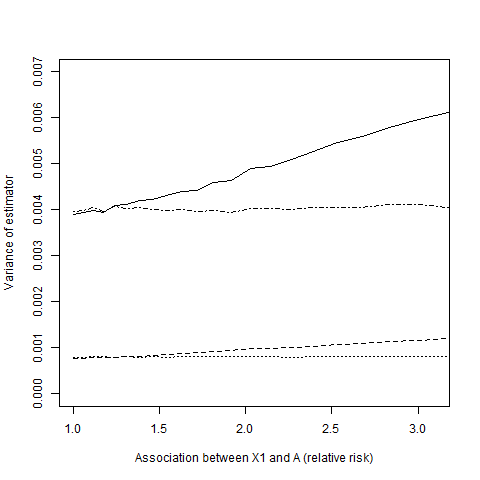
\includegraphics[width=450pt]{../analysis/figures/Figure2} \caption{Replication of Figure 2 in original manuscript. Results are very similar.}\label{fig:unnamed-chunk-1}
\end{figure}
\begin{figure}
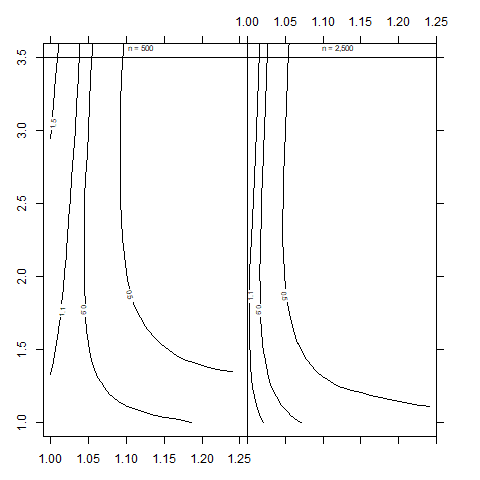
\includegraphics[width=450pt]{../analysis/figures/Figure3} \caption{Replication of Figure 3 in original manuscript. Results are very similar.}\label{fig:unnamed-chunk-2}
\end{figure}
\begin{figure}
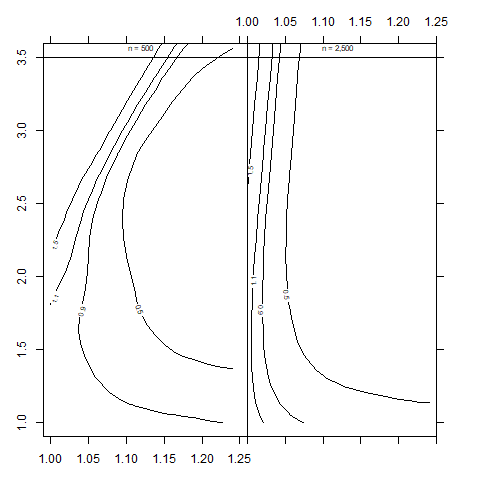
\includegraphics[width=450pt]{../analysis/figures/Figure4} \caption{Replication of Figure 4 in original manuscript. The left panel is different from the original manuscript.}\label{fig:unnamed-chunk-3}
\end{figure}

\FloatBarrier
\section{Discussion}

\subsection{Replicability}

The manuscript by Brookhart and colleagues (Brookhart et al. 2006)
provided a clear description of the simulation approach, which ensured
that replication of the results was fully possible and relatively
straightforward. The authors (likely) implemented default procedures and
provided formulas and a figure to depict the data-generating mechanism,
thereby capturing all relevant information.

\subsection{Replicator degrees of freedom}

The main ``guesses'' that we had to make were about specific
implementations of the procedures. For example, for estimation of the
cubic splines or construction of the x-axis of figures. These decisions
likely have not had a large impact on the results. Making analysis code
available (as is more common nowadays than back in 2006) would have
resolved all issues.\\
Reflecting on the replication process, we found the symmetrical
behaviour of our checks interesting. When we found a result similar to
the maintext, we would continue programming the next part of the
analysis. However, when we ran into a discrepancy, we tried different
implementations (like explained in section 2.6) to obtain the original
result.

\subsection{Equivalence of results}

By and large, the replicated results are equivalent to the original
results. The orders of magnitude and directions are similar and we would
draw the same conclusions based on the results. Figure 4 is the only
aspect we could not fully replicate.

\subsection{Comparison with independent replication team}

\section{Contributions}

Authors made the following contributions according to the CRediT
framework \url{https://casrai.org/credit/}

Primary Replicator:

\begin{itemize}
\tightlist
\item
  Data Curation\\
\item
  Formal Analysis (lead)\\
\item
  Investigation\\
\item
  Software\\
\item
  Visualization (lead)\\
\item
  Writing - Original Draft Preparation\\
\item
  Writing - Review \& Editing
\end{itemize}

Co-Pilot:

\begin{itemize}
\tightlist
\item
  Formal Analysis (supporting)\\
\item
  Investigation\\
\item
  Software (supporting)\\
\item
  Visualization (supporting)\\
\item
  Validation\\
\item
  Writing - Review \& Editing
\end{itemize}

\newpage

\section*{References}
\begingroup
\hphantom{x}
\setlength{\parindent}{-0.5in}
\setlength{\leftskip}{0.5in}

\hypertarget{refs}{}
\leavevmode\hypertarget{ref-brookhart2006variable}{}%
Brookhart, M Alan, Sebastian Schneeweiss, Kenneth J Rothman, Robert J
Glynn, Jerry Avorn, and Til Stürmer. 2006. ``Variable Selection for
Propensity Score Models.'' \emph{American Journal of Epidemiology} 163
(12): 1149--56.

\leavevmode\hypertarget{ref-perperoglou2019review}{}%
Perperoglou, Aris, Willi Sauerbrei, Michal Abrahamowicz, and Matthias
Schmid. 2019. ``A Review of Spline Function Procedures in R.'' \emph{BMC
Medical Research Methodology} 19 (1): 46.

\leavevmode\hypertarget{ref-rougier2017sustainable}{}%
Rougier, Nicolas P, Konrad Hinsen, Frédéric Alexandre, Thomas Arildsen,
Lorena A Barba, Fabien CY Benureau, C Titus Brown, et al. 2017.
``Sustainable Computational Science: The Rescience Initiative.''
\emph{PeerJ Computer Science} 3: e142.

\FloatBarrier
\endgroup
\newpage

\section*{Appendix}

\subsection*{Additional result}

\texttt{\textless{}insert\ additional\ results\ not\ reported\ in\ the\ original\ article\ or\ results\ presented\ in\ an\ alternative\ way\textgreater{}}

\subsection{Code organization}

The code and the files associated are organized in the form of a
research compendium which can be found in the following git repository
\texttt{https://github.com/replisims/Brookhart\_MA-2006/}

\begin{verbatim}
## .
## +-- defs.aux
## +-- defs.tex
## +-- flowchart.PNG
## +-- Lato-Black.ttf
## +-- Lato-BlackItalic.ttf
## +-- Lato-Bold.ttf
## +-- Lato-BoldItalic.ttf
## +-- Lato-Italic.ttf
## +-- Lato-Regular.ttf
## +-- paper.log
## +-- paper.Rmd
## +-- paper.tex
## +-- references.bib
## +-- Replication_notes.pdf
## +-- UbuntuMono-Bold.ttf
## +-- UbuntuMono-BoldItalic.ttf
## +-- UbuntuMono-Italic.ttf
## \-- UbuntuMono-Regular.ttf
\end{verbatim}

\begin{itemize}
\tightlist
\item
  \texttt{foldername}: contains
  \texttt{\textless{}insert\ description\textgreater{}}
\item
  \texttt{filename}: contains
  \texttt{\textless{}insert\ description\textgreater{}}
\item
  \ldots{}
\end{itemize}

\subsubsection*{Reproducibility Information}

This report was last updated on 2020-10-08 18:32:12. The simulation
replication was conducted using the following computational environment
and dependencies:

\FloatBarrier

\begin{verbatim}
## - Session info ---------------------------------------------------------------
##  setting  value                       
##  version  R version 3.6.3 (2020-02-29)
##  os       Windows 10 x64              
##  system   x86_64, mingw32             
##  ui       RTerm                       
##  language (EN)                        
##  collate  Dutch_Netherlands.1252      
##  ctype    Dutch_Netherlands.1252      
##  tz       Europe/Berlin               
##  date     2020-10-08                  
## 
## - Packages -------------------------------------------------------------------
##  package        * version    date       lib
##  assertthat       0.2.1      2019-03-21 [1]
##  backports        1.1.7      2020-05-13 [1]
##  callr            3.4.3      2020-03-28 [1]
##  cli              2.0.2      2020-02-28 [1]
##  crayon           1.3.4      2017-09-16 [1]
##  desc             1.2.0      2018-05-01 [1]
##  devtools         2.3.1      2020-07-21 [1]
##  digest           0.6.25     2020-02-23 [1]
##  dplyr          * 0.8.5      2020-03-07 [1]
##  ellipsis         0.3.1      2020-05-15 [1]
##  evaluate         0.14       2019-05-28 [1]
##  fansi            0.4.1      2020-01-08 [1]
##  fs               1.4.2      2020-06-30 [1]
##  glue             1.4.1      2020-05-13 [1]
##  htmltools        0.5.0      2020-06-16 [1]
##  knitr          * 1.29       2020-06-23 [1]
##  lifecycle        0.2.0      2020-03-06 [1]
##  magrittr         1.5        2014-11-22 [1]
##  memoise          1.1.0      2017-04-21 [1]
##  pillar           1.4.6      2020-07-10 [1]
##  pkgbuild         1.1.0      2020-07-13 [1]
##  pkgconfig        2.0.3      2019-09-22 [1]
##  pkgload          1.1.0      2020-05-29 [1]
##  prettyunits      1.1.1      2020-01-24 [1]
##  processx         3.4.3      2020-07-05 [1]
##  ps               1.3.3      2020-05-08 [1]
##  purrr            0.3.4      2020-04-17 [1]
##  R6               2.4.1      2019-11-12 [1]
##  Rcpp             1.0.5      2020-07-06 [1]
##  remotes          2.2.0      2020-07-21 [1]
##  RepliSimReport   0.0.0.9000 2020-09-28 [1]
##  rlang            0.4.7      2020-07-09 [1]
##  rmarkdown        2.3        2020-06-18 [1]
##  rprojroot        1.3-2      2018-01-03 [1]
##  sessioninfo      1.1.1      2018-11-05 [1]
##  stringi          1.4.6      2020-02-17 [1]
##  stringr          1.4.0      2019-02-10 [1]
##  testthat         2.3.2      2020-03-02 [1]
##  tibble           3.0.3      2020-07-10 [1]
##  tidyselect       1.0.0      2020-01-27 [1]
##  usethis          1.6.1      2020-04-29 [1]
##  vctrs            0.3.2      2020-07-15 [1]
##  withr            2.2.0      2020-04-20 [1]
##  xfun             0.16       2020-07-24 [1]
##  xtable         * 1.8-4      2019-04-21 [1]
##  yaml             2.2.1      2020-02-01 [1]
##  source                                   
##  CRAN (R 3.6.3)                           
##  CRAN (R 3.6.3)                           
##  CRAN (R 3.6.3)                           
##  CRAN (R 3.6.3)                           
##  CRAN (R 3.6.3)                           
##  CRAN (R 3.6.3)                           
##  CRAN (R 3.6.3)                           
##  CRAN (R 3.6.3)                           
##  CRAN (R 3.6.3)                           
##  CRAN (R 3.6.3)                           
##  CRAN (R 3.6.3)                           
##  CRAN (R 3.6.3)                           
##  CRAN (R 3.6.3)                           
##  CRAN (R 3.6.3)                           
##  CRAN (R 3.6.3)                           
##  CRAN (R 3.6.3)                           
##  CRAN (R 3.6.3)                           
##  CRAN (R 3.6.3)                           
##  CRAN (R 3.6.3)                           
##  CRAN (R 3.6.3)                           
##  CRAN (R 3.6.3)                           
##  CRAN (R 3.6.3)                           
##  CRAN (R 3.6.3)                           
##  CRAN (R 3.6.3)                           
##  CRAN (R 3.6.3)                           
##  CRAN (R 3.6.3)                           
##  CRAN (R 3.6.3)                           
##  CRAN (R 3.6.3)                           
##  CRAN (R 3.6.3)                           
##  CRAN (R 3.6.3)                           
##  Github (replisims/RepliSimReport@0cf1ce2)
##  CRAN (R 3.6.3)                           
##  CRAN (R 3.6.3)                           
##  CRAN (R 3.6.3)                           
##  CRAN (R 3.6.3)                           
##  CRAN (R 3.6.2)                           
##  CRAN (R 3.6.3)                           
##  CRAN (R 3.6.3)                           
##  CRAN (R 3.6.3)                           
##  CRAN (R 3.6.3)                           
##  CRAN (R 3.6.3)                           
##  CRAN (R 3.6.3)                           
##  CRAN (R 3.6.3)                           
##  CRAN (R 3.6.3)                           
##  CRAN (R 3.6.3)                           
##  CRAN (R 3.6.2)                           
## 
## [1] C:/Program Files/R/R-3.6.3/library
\end{verbatim}

The current Git commit details are:


\end{document}
